\section{Experiments}

We have measured the overhead of the PCAST OpenACC autocompare implementation to demonstrate its usability.
We used ten of the SPEC ACCEL v1.2 benchmarks, using the \emph{test} dataset.
In each case, the program has an outer time step loop containing the main computation.
The times shown are in seconds, and these are officially SPEC \emph{estimates}, since they were not run in the SPEC harness.
%The host machine was a 6-core Intel Haswell (core i7-5820K) with a 3.30GHz clock, with an NVIDIA Tesla Kepler K40c GPU.
The host machine was a dual socket 16-core Intel Haswell (E5-2698 Xeon, 32-cores total) with a 2.30GHz clock, with an NVIDIA Tesla Pascal P100 GPU.
We used the default autocompare options, but set a relative tolerance.
The execution times are in seconds, measured with /usr/bin/time.
%The values shown in Table~\ref{res1} and Figure~\ref{fig:sle_figure} are:
The values shown in Table~\ref{res1} are:
\begin{itemize}
\item Time to run the test data set sequentially on the CPU.
\item Time to run the test data set in parallel on the GPU.
\item Time to run the test data set redundantly on both CPU and GPU without the autocompare feature enabled.
\item Time to copy the data from GPU to CPU before comparing, measured by nvprof.
\item Time to run the test data set redundantly on both CPU and GPU using the autocompare feature.
\end{itemize}


%\begin{table}
%\begin{center}
%\begin{tabular}{rrrrl}
%\hline
% 303.ostencil & 304.olbm & 363.swim & \\
%\hline
% 3.40s &  3.27s & 1.80s & CPU time (sequential) \\
% 3.27s &  2.79s & 1.72s & GPU time \\
% 8.80s &  3.97s & 1.88s & redundant execution on CPU and GPU \\
% 1.80s &  1.69s & 0.09s & CPU to GPU data copy time \\
%64.38s & 23.95s & 2.80s & autocompare time \\
%202 & 61 & 258 & variables and arrays compared \\
%3,388,997,632 & 1,586,800,000 & 67,897,602 & values compared \\
%\hline
%\end{tabular}
%\end{center}
%\caption{Results showing overhead of OpenACC autocompare.}
%\label{res1}
%\end{table}

\begin{table}
\begin{center}
\begin{tabular}{|l|c|c|c|c|c|c|c|c|c|}
\hline

Benchmark & \parbox[c]{1.9 cm}{\centering CPU time \\(sequential)} &  \parbox[c]{1 cm}{\centering GPU \\ time} & \parbox[c]{3.5 cm}{\centering Redundant execution \\ on CPU and GPU} & \parbox[c]{2.75 cm}{\centering CPU to GPU \\  data copy time} &  \parbox[c]{2 cm}{\centering Autocompare \\   time} \\



\hline
%303.ostencil  & 3.40s & 3.25s & 4.34s & 1.14s & 17.58s \\
%304.olbm      & 2.44s & 1.54s & 3.20s & 0.96s & 22.32s \\
%363.swim      & 1.64s & 1.13s & 1.15s & 0.04s & 2.06s \\

ostencil  & 3.51 & 1.82 & 4.22 & 1.03 & 17.19\\
olbm      & 2.19 & 1.30 & 3.03 & 0.96 & 19.09 \\
omriq     & 1.49 & 0.88 & 2.05 & 0.03 & 2.08\\
palm      & 2.75 & 1.45 & 3.75 & 0.50 & 15.75\\
ep        & 2.50 & 0.98 & 3.19 & 0.11 & 3.21\\
miniGhost & 0.87 & 1.07 & 1.69 & 1.23 & 13.17\\
cg        & 62.98 & 28.74 & 64.86 & 0.28 & 68.43\\
csp       & 2.78 & 1.20	& 3.64 & 26.69 & 309.99\\
ilbdc     & 160.62 & 2.10 & 160.39 & 27.41 & 615.26\\
bt        & 5.92 & 1.27 & 7.27 & 9.13 & 119.28\\

            
\hline
\end{tabular}
\end{center}
\caption{Results showing overhead of the PCAST OpenACC autocompare feature.}
\label{res1}
\end{table}


In Table~\ref{res2} 
We show some statistics about the benchmarks we used, such as:
\begin{itemize}
\item Number of variables or arrays compared.
\item Number of data values compared.
\item Number of variables or arrays that had some differences.
\item Number of data values that were different.
\end{itemize}




\begin{table}
\begin{center}
\begin{tabular}{|l|c|c|c|c|c|c|c|c|c|}
\hline

Benchmark &  \parbox[c]{3 cm}{\centering Variables and \\ arrays compared} &  \parbox[c]{2 cm}{\centering Values \\ compared} &  \parbox[c]{3 cm}{\centering variables and arrays \\     with differences} & \parbox[c]{2 cm}{\centering Differences \\      tolerated}\\



\hline
%303.ostencil & 202 & 3,388,997,632 & 0 & 0 \\
%304.olbm     & 61 & 1,586,800,000 & 59 & 520,634,266 \\
%363.swim     & 259 & 67,897,602 & 259 & 22,336,658 \\

ostencil  & 202 & 3388997632 & 0 & 0\\
olbm      & 61 & 586800000 & 59 & 520634266\\
omriq     & 3 & 68608 & 2 & 53240 \\
palm      & 31244 & 1532482935 & 14784 & 374679922\\
ep        & 4 & 13 & 2 & 2 \\
miniGhost & 2506 & 1844059545 & 175 & 175\\
cg        & 186 & 621600195 & 168 & 4858272\\
csp       & 4057 & 40132155677	& 3897 & 5693059\\
ilbdc     & 3001 & 53818895200 & 2000 & 35305830600 \\
bt        & 5036 & 15041440200 & 4798 & 38931891 \\

            
\hline
\end{tabular}
\end{center}
\caption{Results showing number of variables PCAST OpenACC autocompare feature processed.}
\label{res2}
\end{table}




Figure~\ref{fig:sle_figure} breaks down the time spent in the autocompare run into:
\begin{itemize}
\item Compute Time: the max of the CPU time and GPU time from Table~\ref{res1}.
\item Redundancy Overhead: the difference between the redundant execution time from Table~\ref{res1} and Compute Time.
\item Download Time: the time spent downloading data as measured using nvprof.
\item Compare Time: the difference between autocompare time from Table~\ref{res1} and the sum of the above three times.
\end{itemize}

%\begin{figure*}[t]
%    \centering
%    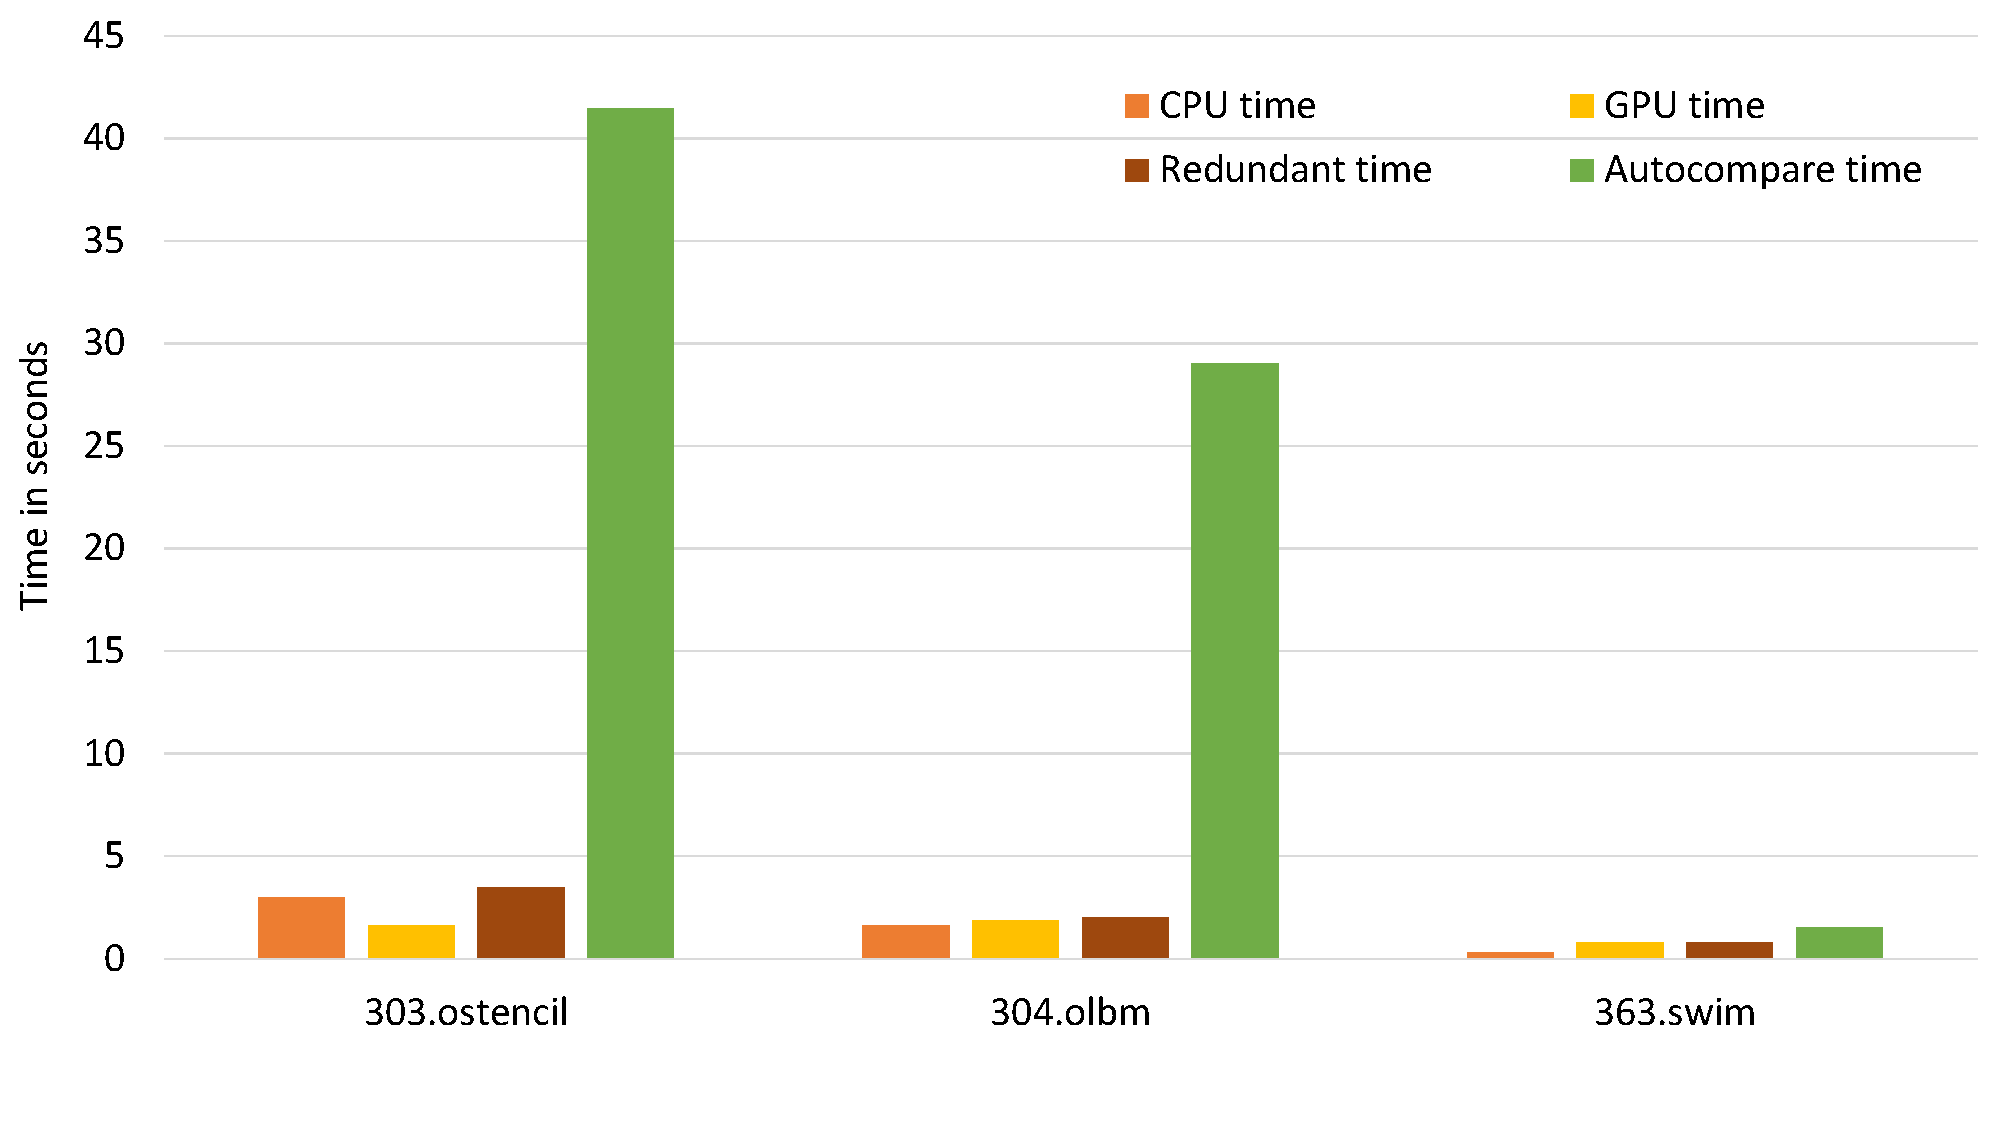
\includegraphics [width=1\linewidth] {Table1.pdf}
%    \caption{Results showing overhead of the PCAST OpenACC autocompare feature.}
%    \label{fig:sle_figure}
%\end{figure*}

\begin{figure*}[t]
    \centering
    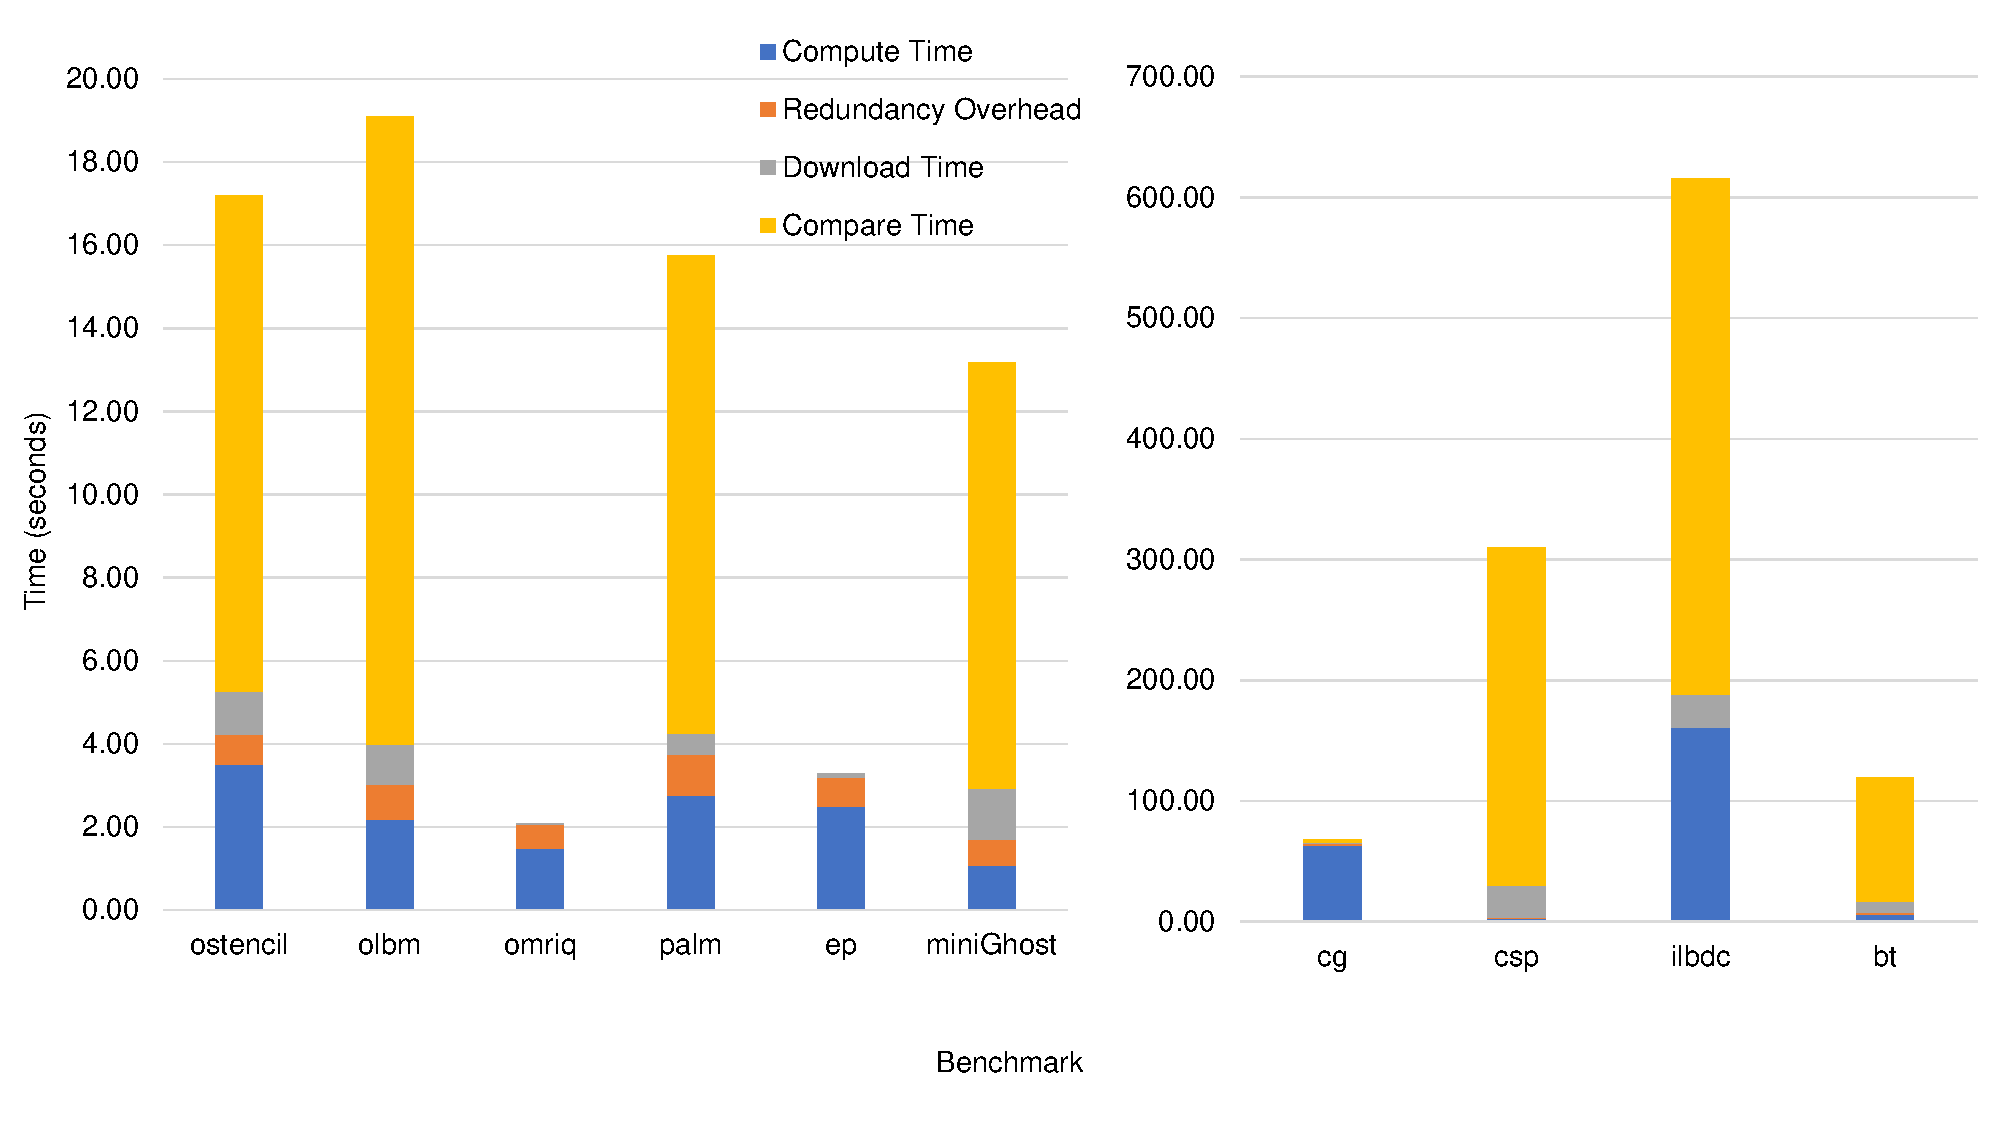
\includegraphics [width=1\linewidth] {npic3.pdf}
    \caption{Results showing overhead of the PCAST OpenACC autocompare feature.}
    \label{fig:sle_figure}
\end{figure*}


The costs of the autocompare feature are running the compute region on both CPU and GPU, and downloading and comparing the values.
The cost of redundant execution is less than the sum of the CPU and GPU times, because the GPU code executes asynchronously while the CPU executes the corresponding code.
Since this is a feature used during code development and debugging, we consider this to be relatively low overhead.
The cost of doing the many floating point comparisons is significant, and seems directly related to the number of data items compared, and unrelated to the number of arrays or variables being compared.
However, using this feature to find where a GPU computation diverges moves the cost from the programmer to the computer, so it could be invaluable regardless of the overhead. An interesting observation we came across was that on all benchmarks we used it roughly took one second to compare a gigabyte of data as can be seen in figure ~\ref{fig:gbps_figure}, which can be used as a rough estimate of how long it will take to test a code for correctness as long as the user knows the size of the data set being used.

\begin{figure*}[t]
    \centering
    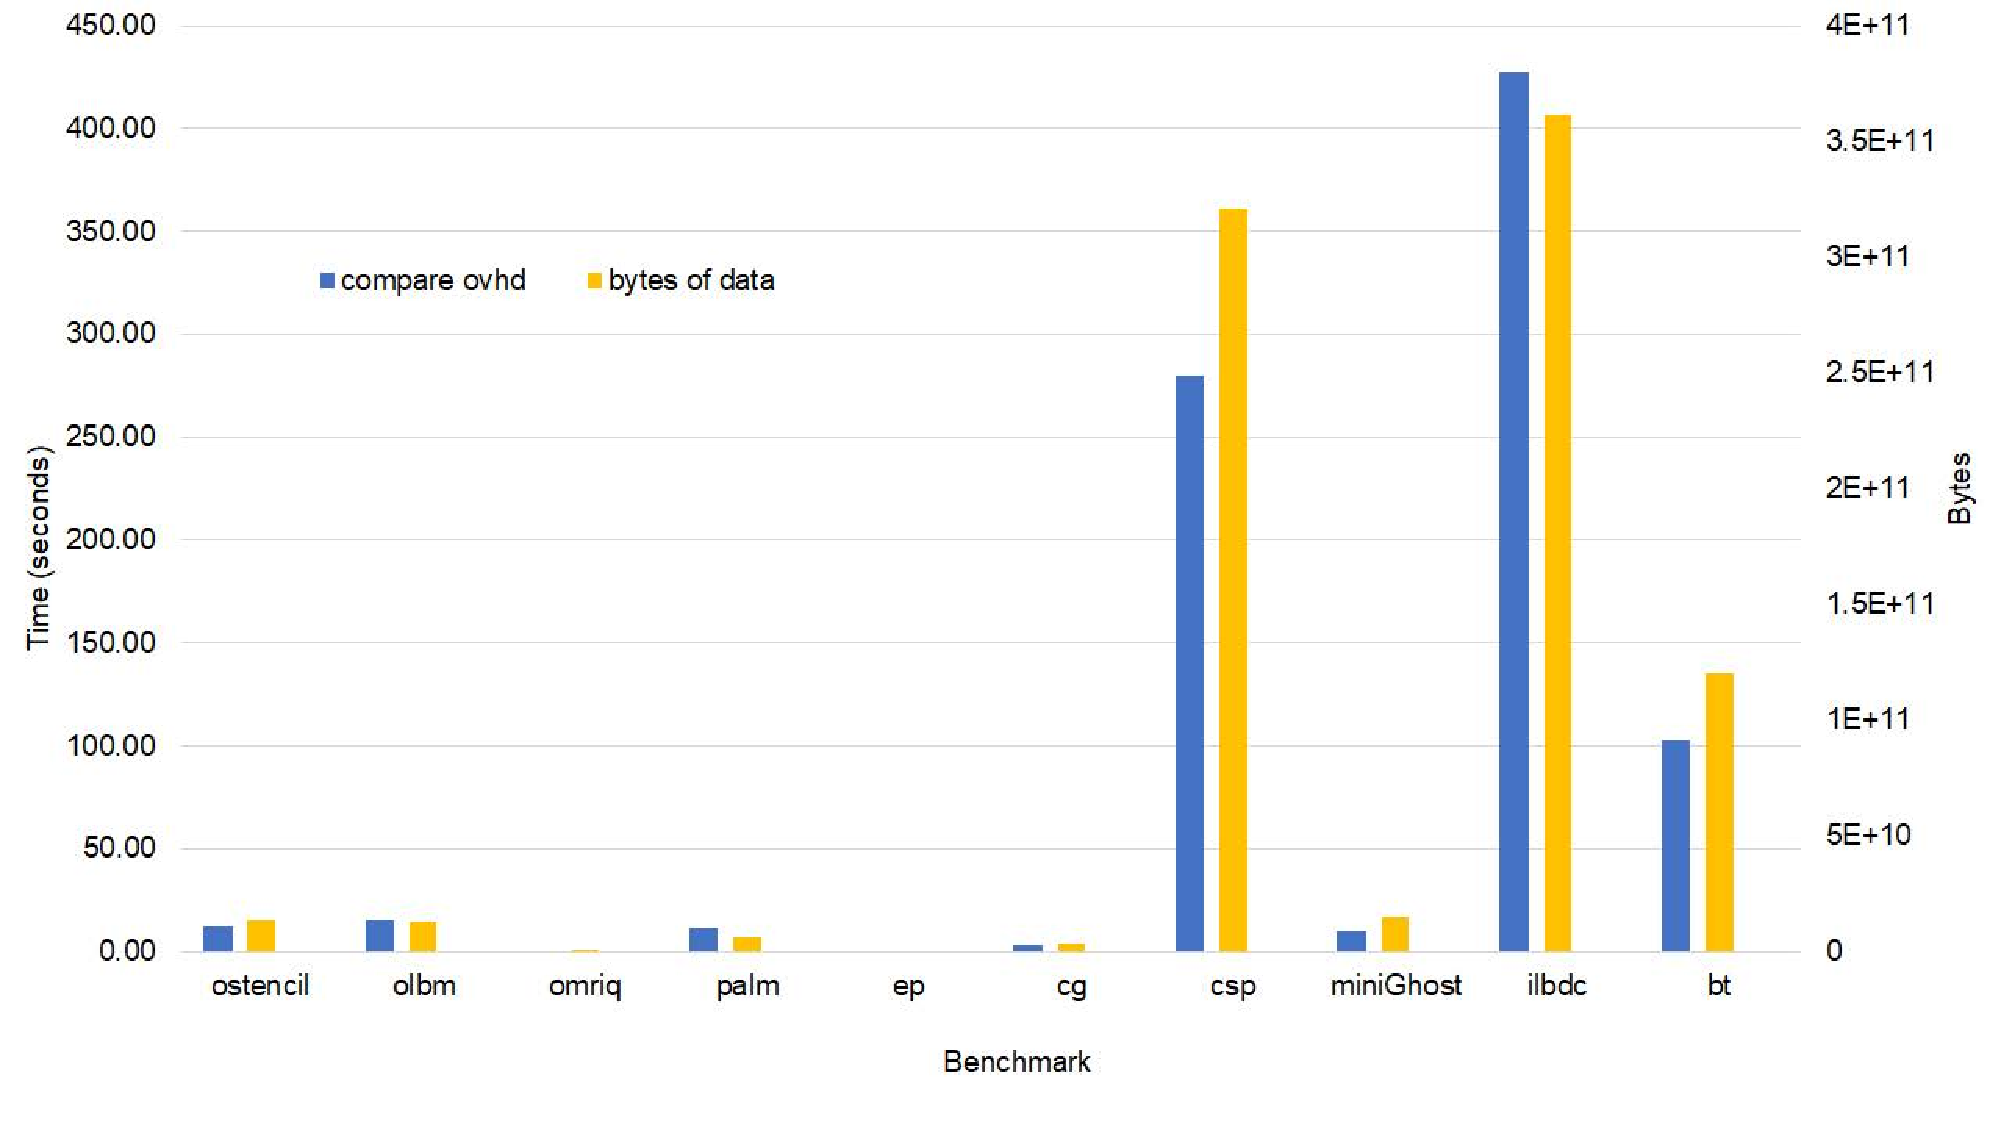
\includegraphics [width=1\linewidth] {GBperSec.pdf}
    \caption{Results showing amount of data the autocompare feature process per unit time.}
    \label{fig:gbps_figure}
\end{figure*}

One side note: the \emph{test} datasets used here are relatively small.
Even so, we had to set the relative tolerance to avoid the comparisons detecting differences, mostly due to different summation accumulation order.
Surprisingly, those differences propagated to about $\frac{1}{3}$ of the results in two of the ten benchmarks that we show here.
This seems to imply that the cost of computing and comparing a quick checksum or signature before downloading and comparing all the data would frequently have little or no benefit.
